In this chapter, we present our approach in transforming BPMN 2 models into Reo networks. Since the core of Extensible Coordination Tool-set (ECT) \cite{ect} and Eclipse BPMN 2 modeler \cite{activiti} are based on Eclipse Modeling Framework (EMF) \cite{emf}, the BPMN 2 to Reo transformation can be carried out in the {model-driven} paradigm. We use the Eclipse de-facto model transformation language and toolkit called Atlas Transformation Language (ATL) \cite{atl}. 

ATL is a high level rule-based language dedicated to model transformation. By using ATL we benefit from the power of separation of concerns and focus only on the required mapping rules, rather than matching patterns on the source models and execution of the rules. 

The mapping rules presented in this chapter are mainly based on the conceptual mapping of BPMN primitives to Reo presented in \cite{bpmn2reo} \cite{AS08}. The following is a brief summary of the mapping:

\begin{itemize}
 \item A task or a collapsed sub-process is mapped to a $FIFO_1$ channel, which denotes a unit of work in a process. However, an  expanded sub-processes is modeled using a Reo connector whose inner elements are mapped from the inner elements of the sub-process.
 
 \item In general, an event is mapped to a replicator node. For each start event, a writer is created and connected to a source end of the node to simulate the arrival of the event. Similarly, each end event is connected to a reader on one of its sink ends. Throwing events are connected to the corresponding catching events using $FIFO_1$ and lossySync channels. So, they do not block the flow in case that the catching events are not yet ready to receive the event.
 \begin{itemize}
               \item For each conditional event, a filter channel with the corresponding condition is created and connected to the source end of the node. %So, it appdirects the flow from the previous element in the 
               %\item Message Signal
              % \item timer??
               \item The terminate and throwing compensation are special cases, which their mappings requires possible compensations. Therefore, they have more sophisticated mappings, which we discuss in this chapter. %while mapping transactions.??
\end{itemize}

 \item Gateways are mapped to different kinds of Reo nodes based on their types and the number of their incoming and outgoing sequence flows.
 \begin{itemize}
  \item A data-based exclusive gateway is mapped to a router node, while each of its outgoing sequence flows is mapped to a filter channel with a corresponding condition.  
  \item A data-based inclusive gateway is mapped to a replicator node.  
  \item A parallel event-based gateway with one incoming flow is mapped to a replicator. In case that it has more than one incoming flows, it is mapped to a join node.
\end{itemize}

 \item Sequence and message flows are mapped to synchronous channels unless there exists a more specific rule that describes the mapping in a given context. %, as presented above. %few cases.?? %In that case,  rule is used
\end{itemize}

Most BPMN 2 elements can be mapped to Reo constructs, which have relatively similar granularity. One notable exception is that mapping of transactions requires more effort than the other BPMN 2 elements do, and it creates many more Reo constructs. 
This is due to the complex behavior of BPMN 2 transactions compared to the other elements. 

Tasks in a transaction should be compensated in the reverse order of their execution. In addition, the post compensation flow cannot be taken unless all performed compensatable tasks are compensated. Addressing these concerns requires more elements to be added to the target model.
 
Since for mapping transactions requires more work compared with the rest of elements. We refine them with groups of finer grained elements, which collectively deliver the same functionality. This is done prior to performing the transformation.

The rest of this chapter is organized as follows: Section \ref{sec:refine} presents an algorithm to refine BPMN 2 transactions in order to simplify the mapping procedure. Section \ref{sec:atl} is a brief introduction to Atlas Transformation Language (ATL). Our proposed BPMN 2 to Reo mapping is given in Section \ref{sec:b2r}. We show result of the mapping using an example in Section \ref{exmap}. Section \ref{chapterconv:relwrk} overviews the related work on transformation of BPMN models. 

\section{Transaction refinement}
\label{sec:refine}
To simplify mapping of BPMN transactions, we substitute them with a set of BPMN 2 elements that are easier to map to Reo, yet collectively expose the same functionality. % (in terms of the performed activities and their order). 
The correctness of this refinement can be checked against the informal behavioral description of the elements involved. We do not provide a formal proof. 

The mechanism to trigger a compensation in BPMN 2 is either by using a cancel event attached to the boundary of a transaction  or by throwing a compensation event.   
For simplicity, we assume that all compensations are triggered in the former way. It is not a limiting assumption as it is possible to convert the latter to the former. 

In the refinement process, we create complex gateways for two purposes: i) to control the execution order of compensation tasks and ii) to delay the post compensation flow. We refer to them as {compensation order} and {post compensation}, respectively. 

We use these complex gateways as placeholders to be replaced by groups of Reo elements, which implement the informally described behavior of the gateways. Though the behavior of complex gateway is defined by its {expression} attribute, for these gateways, we ignore their expression attribute. During the refinement process, though, we keep track of these gateways and pass their identifiers to the ATL mapping process in order to invoke the suitable mapping rules. 

We carry out the refinement as follows:

\begin{enumerate}
\item We create a send signal event for each compensatable task and place it after the task (using an inclusive gateway if the task has a following element). This is to notify when the task is completed.
\item When a compensatable task resides in a sequence of compensatable tasks, only the last performed task can be compensated immediately upon receiving the cancel event. The rest of the tasks should be compensated only if their following tasks in the sequence are compensated. Therefore, for each compensatable task in a sequence except for the last task, we create a send signal event and place it after the compensation task corresponding to that task (using gateways for connecting objects when it is necessary). These events are fired after the corresponding compensatable tasks are compensated.
\item For a compensatable task $T_a$ with a following compensatable task $T_b$ in a sequence of compensatable tasks, we create a {complex gateway} (of type compensation order) with incoming sequence flows originating from 1) the {cancel boundary event}, 2) a newly created {receive signal event}, which catches the signal corresponding to completion of $T_a$, 3) a newly created {receive signal event}, which catches the signal corresponding to completion of $T_b$, and 4) a newly created {receive signal event}, which catches the signal corresponding to completion of the compensation of $T_b$. The {complex gateway} sends flow to the {compensation task} corresponding to $T_a$ only if all incoming sequence flows are enabled. 
\end{enumerate}

The above steps assure that the compensation tasks are invoked in the right order. In addition, we need to prevent that the outgoing sequence flow of the cancel boundary event is taken before all compensation tasks within the given transaction are completed. The following step realizes this.

\begin{enumerate}
  \setcounter{enumi}{3}
\item Let $c_e$ be the cancel boundary event of the given transaction, $s_e$ be the outgoing sequence flow of $c_e$, and  $f_e$ be the target of $s_e$. We create a new complex gateway $g_e$ (of type post compensation) and remove $s_e$. For each compensation task $t_c$ and its corresponding componsatable task $t_a$, we create a new receive signal event to receive these signals. For each event, we create a sequence flow, which has the event as its source and $g_c$ as its target. This complex gateway enables its outgoing sequence flow if the cancel event is received and after receiving each receive signal event corresponding to the compensatable task $t_a$, the receive signal event corresponding to the compensation of the task $t_c$ is received, as well.
\end{enumerate}

Listings \ref{lst:nrefine}, \ref{lst:nrefine2}, and \ref{lst:nrefine3} depict our algorithm for transaction refinement. To reduce verbosity, we provide the following definitions:

\begin{itemize}
\item The \emph{objects} property of a transaction is the set of its enclosed BPMN 2 flow objects (i.e. activities, gateways, and events).
\item The \emph{compensation} property refers to the {compensation} task corresponding to the activity. If the {task} is not compensatable, this value is \emph{null}.
\item The \emph{nextFlowObjects} property is the set of all the flow objects that are directly connected to an outgoing sequence flow from the flow object.
\item The \emph{previousFlowObjects} property is the set of all the flow objects that are directly connected to an incoming sequence flow from the flow object.
\item The \emph{receivers}, a property of a {send signal event}, is the set of the receivers of the event. 
\item The \emph{getDoneSignal} function maps a {compensatable} or a {compensation} task to their corresponding {send signal event}.
\item The \emph{getNextCompensatables} function maps a {compensatable task} to its following {compensatable tasks} in sequences of {compensatable tasks} if they exist. Otherwise, it returns \emph{null}.   
\end{itemize}

In addition, we assume that adding an {object} to the {nextFlowObjects} list creates the required connecting objects.

%\newpage
\begin{lstlisting}[float,numbers=left,numbersep=5pt,mathescape=true,caption=Refinement of transactions,label=lst:nrefine]
refine(BPMN2Process proc) {
  foreach (Transaction tran in proc.objects.filter(e | e.isTypeOf(`Transaction'))) {
  
    Event[] cancels = tran.objects.filter(e | e.isTypeOf(`CatchingCancelEvent'));
    assert(cancels.length == 1);
    
    Gateway postCompensation = new ComplexGateway();
    postCompensation.nextFlowObjects = cancels[0].nextFlowObjects;
    cancels[0].nextFlowObjects = {postCompensation};
    
    foreach(Task start : tran.objects.filter(e | e.isTypeOf(`Task') $\wedge$ e.compensation != null) and tran.previousFlowObjects().length == 0) {
    
        // Allow post compensation flow only when all performed compensatable tasks are compensated
        Event taskDone = new CatchingSignalEvent();
        getDoneSignal(task).receivers.add(taskDone);
        taskDone.nextFlowObjects = {postCompensation};
        
        Event compensationDone = new CatchingSignalEvent();
        getDoneSignal(task.compensation).receivers.add(compensationDone);
        compensationDone.nextFlowObjects = {postCompensation};
    }
    
    foreach (CompensatableTask task in tran.objects.filter(e | e.isTypeOf(`Task') $\wedge$ e.compensation != null)) {
        handleTaskCompletion(task);
        handleCompensation(cancels[0], task);
    }
  }
}
\end{lstlisting}
\begin{lstlisting}[float,numbers=left,numbersep=5pt,mathescape=true,caption=Refinement of transactions (dealing with task completion),label=lst:nrefine2]
handleTaskCompletion(CompensatableTask task) {
  // A send signal event to indicate the task is done
  Event doneSendEvent = new SendSignalEvent();
  // A receive signal event to catch the signal above
  Event doneReceiveEvent = new CatchingSignalEvent();  
  doneSendEvent.receivers = {doneReceiveEvent};
  // Placing the signal event after the task
  if (task.nextFlowObjects == null) {
    task.nextFlowObjects = {doneSendEvent};
  } else {
    Gateway gateway = new InclusiveGateway();
    gateway.nextFlowObjects = task.nextFlowObjects;
    gateway.nextFlowObjects.add(doneSendEvent);
    task.nextFlowObjects = {gateway};
  }
}
\end{lstlisting}
\begin{lstlisting}[float,numbers=left,numbersep=5pt,mathescape=true,caption=Refinement of transactions (dealing with compensations),label=lst:nrefine3]
handleCompensation(CatchingCancelEvent cancel, CompensatableTask task) {
  Event receiver = getDoneSignal(task).receivers[0];
  CompensatableTask[] nexts = getNextCompensatables(task);
  if (nexts.length == 0) {
    Gateway gateway = new InclusiveGateway();
    cancel.nextFlowObjects.add(gateway);
    receiver.nextFlowObjects = {gateway};
    gateway.nextFlowObjects.add(task.compensation);
  } else {
    // A complex gateway that fires if either all or 
    // only the first two of its inputs have flow
    Gateway order = new ComplexGateway();
    cancel.nextFlowObjects.add(order);
    receiver.nextFlowObjects.add(order);
    
    foreach(CompensatableTask next in nexts) {
      // Event associated with the next compensatable task
      getDoneSignal(next).nextFlowObjects.add(order);
    
      // Event associated with compensation of the next
      // compensatable task
      Event compensationDone = getDoneSignal(next.compensation).receivers[0];
      getDoneSignal(compensationDone).nextFlowObjects.add(order);
    }
    order.nextFlowObjects.add(receiver);
  }
}
\end{lstlisting}

The refinement starts with the {refine} method, which goes through the {transactions} in a given {process} and asserts that they have a single {catching cancel boundary event}. If the {event} is found, a post compensation complex gateway is created in order to delay the activation of the outgoing sequence flow from the cancel boundary event until all performed compensatable tasks inside the transaction are compensated. Then, for each {compensatable task} the {handleTaskCompletion} and {handleCompensation} methods are invoked.

The {handleTaskCompletion} method creates a {send signal event} and places it after the given {compensatable task} (using a newly created {gateway} to connect it to the other elements if it is needed). Additionally, it creates a {receive signal event} to catch the generated {signal event} and adds it to the {receivers} attribute of the {send signal event}.

The {handleCompensation} method starts by finding the {receive signal event}, which indicates the completion of the given {compensatable task}. Then, it finds the {compensatable tasks} that are immediate successors of the current {compensatable task} within sequences of {compensatable tasks} and creates the signal events described in the third step. 

%In case that the {task} does not reside in any sequence of {compensatable tasks} or it has no following {compensatable task} in such a sequence, it creates a {join gateway} to merge flows from the {cancel event} and the {receive signal event}, which indicates the completion of the {task}, and places it before the corresponding {compensation task}. 
%
%Otherwise, it creates a {complex gateway} with incoming sequence flows from 1) the {cancel boundary event}, 2) the {receive signal event}, which indicates compensation of the task, 3) {receive signal events} indicating completion of the immediate {compensatable successors tasks}, and 4) {receive signal events} indicating completion of compensation for each immediate {compensatable successors task}.  

Figure \ref{fig:baxtionref} demonstrates the result of applying the transaction refinement algorithm on a sample transaction shown in Figure \ref{fig:baxtion}. 

\begin{figure}
%\centering
\subfloat[An example of BPMN 2 transaction (modified from \cite{BPMN20})\label{fig:baxtion}]{
  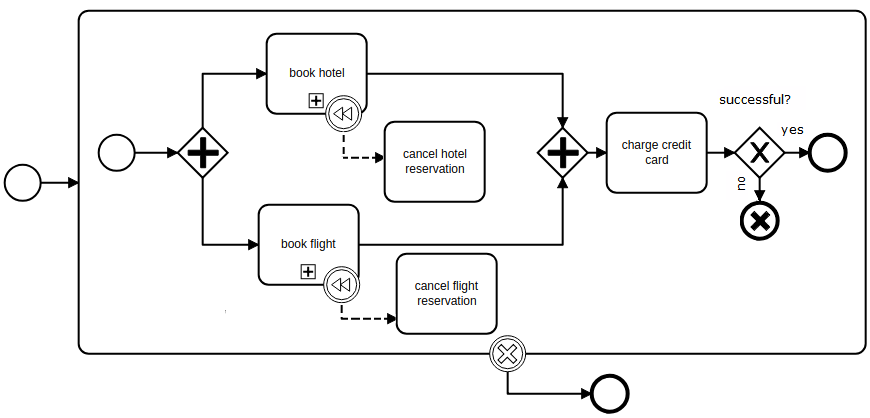
\includegraphics[width=\textwidth]{img/xactionwitresized2.png}
    %\caption{An example of BPMN 2 transaction (modified from \cite{BPMN20})\newline}
}

%  \subfloat[caption fig (a).]{\includegraphics[width=7cm]{<fig1>}\label{fig1}}
\subfloat[Refined transaction\label{fig:baxtionref}]{
  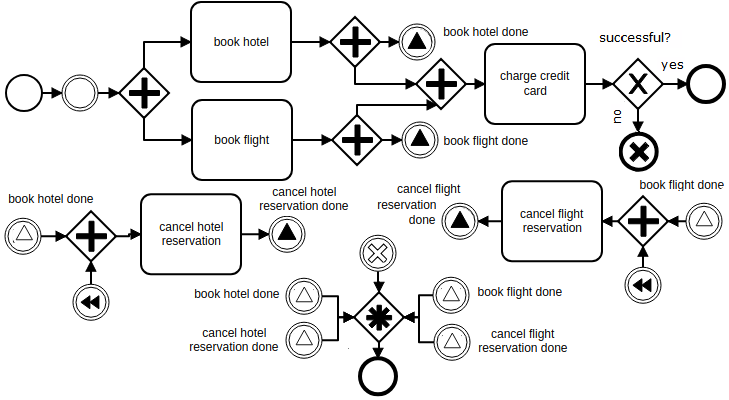
\includegraphics[width=0.9\textwidth]{img/bch-refined-example-2n.png}
%    \caption{Refined transaction}
%    \label{fig:baxtionref}
}
\caption[Figure \ref{fig:baxtion} after refinement]{BPMN 2 model of Figure \ref{fig:baxtion} after performing the transaction refinement}
\label{fig:refinedbahbah}
\end{figure}

\section{Atlas Transformation Language}
\label{sec:atl}
We have implemented the BPMN 2 to Reo transformation in ATL (ATLAS Transformation Language), which is
developed as a part of the ATLAS Model Management Architecture (AMMA)
platform \cite{AMMA}. ATL is a hybrid language, meaning that it supports both declarative and imperative programming styles.

A program in ATL consists of several rules that match against the source model elements and generate target elements.
Rules in ATL are of three types: {matched} and {lazy} rules that are declarative, {called} rules, which  are imperative.

 The matched rules define matching conditions for generating target elements out of the source elements and the way to initialize them from the matched source model element. 
A matched rule contains two mandatory sections, which are the matching and generation patterns; and two optional parts that are local variables definitions and an imperative section. 

Local variables are defined by the keyword {using}. The scope of a local variable is its enclosing rule. The source pattern of a matched rule is defined using the {from} keyword. By defining an expression on the matching pattern, it is possible to restrict the matching of the source elements to those of choice. 
 A source model element of an ATL transformation can only be matched by one  matched rule. 

The optional imperative section is defined by the keyword {do}.
 The generation part of the rule is specified by the {to} keyword. 
 Unlike {matched} rules, a {lazy} rule is only fired when it is called through another rule. 

Imperative programming in ATL is feasible %(but less encouraged) 
using {called} rules. They can accept parameters. In order to run a {called} rule, they need to be explicitly called from an imperative code section.

ATL allows developers to define auxiliary methods, called {helper}s, which can be called from different parts of the program. An ATL helper consists of a {name}, a {context} type, a return type, an ATL expression defining the logic of the {helper}, and an optional set of parameters defined as pairs of $parameter\ name$ and $parameter\ type$.

\begin{lstlisting}[float,frame=single,caption=Definition mapping rule,label=lst:def2mod]  
rule mapDefinition {
  from
    def : BPMN2!Definitions
  to
    mod : Reo!Module(
        name <- def.name, 
        connectors <- def.rootElements->select(e | e.oclIsKindOf(BPMN2!Process))
        )
} 
\end{lstlisting}

\section{Mapping BPMN 2 to Reo}
\label{sec:b2r}
We express the mapping in terms of the BPMN 2 and Reo meta-models. Meta-models provide a precise and systematic way to describe valid models.

The conversion begins by matching the BPMN 2 top most element, which according to the  BPMN 2 meta-model is {Definition}. {Definition} is a container for other BPMN 2 elements.

 Similarly, a {module} serves as the top most container for Reo elements. Both {definition} and {module} can be seen as logical elements that are added in the meta-models in order to preserve the process structure. Neither of them exists in the conceptual definition of the notations. 
 
 \newpage
\begin{lstlisting}[frame=single, caption=Process mapping rule,label=lst:proc2conn]
helper context BPMN2!SubProcess def : expanded : Boolean =
  self.flowElements.size() > 0; 

helper context BPMN2!FlowNode def : expandedSubProcess : Boolean =
  if not self.oclIsKindOf(BPMN2!SubProcess) 
  then false
  else self.expanded
  endif; 

rule mapProcess {
  from
    proc : BPMN2!Process
  to 
    conn : Reo!Connector(
      name <- proc.name, 
      nodes <- proc.flowElements->select(e | e.oclIsTypeOf(BPMN2!Activity) or  e.oclIsTypeOf(BPMN2!Event) or e.oclIsTypeOf(BPMN2!Gateway)), 
      primitives <- proc.flowElements->select(e | e.oclIsTypeOf(BPMN2!SequenceFlow) or (e.oclIsKindOf(BPMN2!SubProcess) and not e.expanded())),
      subConnectors <- proc.flowElements->select(e | e.expandedSubProcess())
    )
}
\end{lstlisting} 
 
\subsection{Definition}
We map a {definition} to a Reo {module}. The rule in Listing \ref{lst:def2mod} carries out this mapping. Similar to all of our mapping rules, it respects the nesting of elements, meaning that the result of mapping an enclosed element is assigned to the mapped parent element. The rule creates a Reo {module} for the BPMN 2 {definition} and triggers rules matching the nested {process}es. The result of the triggered rules will be assigned to {connector}s inside the created {module}. 

The {select} command in the rule collects the {process}es from the list of elements nested within the {rootElements} attribute of the definition.
{RootElement} is an abstract type with {Process} as one of its subtypes. The {select} command applied on {rootElement} guarantees that not any other subtype but {process} will go through this assignment. 

The function {oclIsKindOf} returns \emph{true}, if it is invoked from  either an instance of the passed type or an instance of one of its subtypes. Similarly, the function {oclIsTypeOf} returns \emph{true}, if the element to which it is applied is an instance of the passed type.

\begin{figure}[!t]
  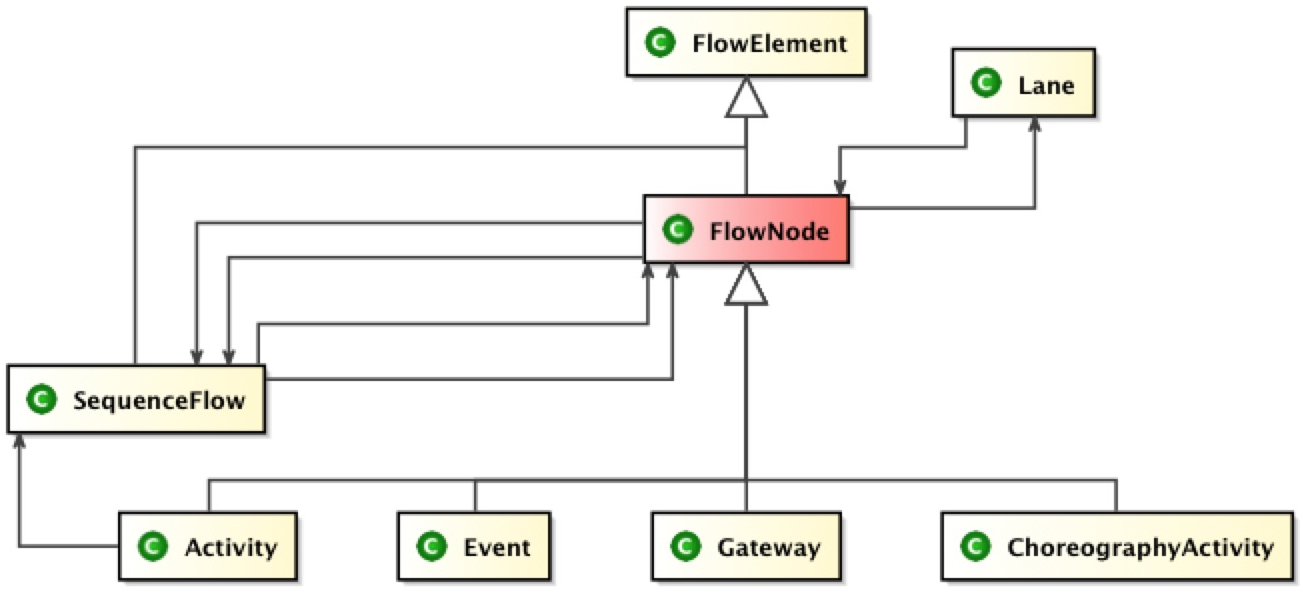
\includegraphics[width=.95\linewidth]{img/emf-flownode}
  \caption[The meta-model of {FlowNode}]{The {FlowNode} and its related entities in BPMN 2 EMF meta-model }
  \label{fig:emfflownode}
\end{figure}

\subsection{Process}
We map a BPMN 2 {process} to a Reo {connector} in Listing \ref{lst:proc2conn}. Besides creating a {connector}, the rule initiates the set of {node}s, {primitive}s, and {subconnector}s from the result of mapping the {activity}, {gateway}, and {event} elements, {sequenceFlow}s, and {subprocess}es, respectively. 

When a mapping rule maps an BPMN 2 elements to a mixture of Reo nodes and primitives those types that are the rules in Listing \ref{lst:proc2conn} does assign to the corresponding attribute in the Reo connector need to be manually assigned to their target attribute of the connector. This is done in the {do} section of those rules, where we place the recently created primitives inside the corresponding Reo connector. Otherwise, these primitives would be floating inside the model.

We assume that a subprocess is collapsed when it has no inner element. The helper {expanded} returns \emph{true}, when it is applied on a subprocess with at least one inner element. The helper {expandedSubProcess} serves the same purpose, but with a difference that it is applicable on any flowNode.

As Figure \ref{fig:emfflownode} demonstrates {FlowNode} mentioned in the rule is the super type of  {activity}, {gateway}, and {event} types in the BPMN 2 meta-model. 

\subsection{Task and subprocess}
Since a BPMN 2 {task} represents one unit of work in a process, we map it to a {FIFO}$_1$ channel while preserving its incoming and outgoing sequence flows. %With the help of pre-processing performed in the transaction refinement, even if a task resides inside a transaction, it does not require a different ATL mapping rule to handle its compensation scenario. 
%Instead, BPMN 2 elements created for realizing compensation are mapped to Reo elements, which together carry out the compensafromcomplexgwtype1hlprtion. 


\begin{lstlisting}[float,frame=single, caption=Mapping tasks and collapsed subprocesses,label=lst:colsubproc]
rule mapTaskAndCollapsedSubprocess {
  from
    nod : BPMN2!FlowNode(nod.oclIsKindOf(BPMN2!Task) or (nod.oclIsKindOf(BPMN2!SubProcess) and not nod.expandedSubProcess()))
  to
    ndc : Reo!Node,
    fif : Reo!FIFO(sourceEnds <- src, sinkEnds <- snk),
    src : Reo!SourceEnd(node <- ndc),
    snk : Reo!SinkEnd(node <- ndk),
    ndk : Reo!Node 
  do {  
    ndc.connector.primitives.add(fif);
  }
}
\end{lstlisting}


Similarly, a collapsed {subprocess} represents a single step in a process by abstracting away from its inner structure, it resembles a Reo {FIFO}$_1$ channel.               Listing \ref{lst:colsubproc} describes the mapping rule for a simple {activity} and a collapsed subprocess. 

\begin{lstlisting}[float,frame=single, caption=Mapping an expanded subprocess,label=lst:nestsubproc2subcon]
rule mapExpandedSubprocess {
  from
    subp : BPMN2!SubProcess(subp.expandedSubProcess())
  to
    conn : Reo!Connector(
       name <- subp.name, 
       nodes <- subp.flowElements->select(e | e.oclIsTypeOf(BPMN2!Task) or e.oclIsTypeOf(BPMN2!Event) or e.oclIsTypeOf(BPMN2!Gateway)),   
       primitives <- subp.flowElements->select(e |  e.oclIsTypeOf(BPMN2!SequenceFlow) or (e.oclIsKindOf(BPMN2!SubProcess) and not e.expandedSubProcess())),
       connector <- subp.flowElements->select(e | e.expandedSubProcess()
    )
}
\end{lstlisting}


%\subsection{Expanded Subprocess}
Unlike a collapsed {subprocess}, an expanded {subprocess} reveals its inner structure. Therefore, we map an expanded subprocess to a Reo {subconnector} that contains Reo elements mapped from the inner elements of the source {subprocess}.  

The rule in Listing \ref{lst:nestsubproc2subcon} first creates a Reo {connector}, then invokes other rules to map its inner elements, and assigns the result to the generated {connector}. 

\subsection{Throw and catch events}
\begin{lstlisting}[float,frame=single, caption=Mapping tasks and collapsed subprocesses,label=lst:colsubproc]
rule mapTaskAndCollapsedSubprocess {
  from
    nod : BPMN2!FlowNode(nod.oclIsKindOf(BPMN2!Task) or (nod.oclIsKindOf(BPMN2!SubProcess) and not nod.expandedSubProcess()))
  to
    ndc : Reo!Node,
    fif : Reo!FIFO(sourceEnds <- src, sinkEnds <- snk),
    src : Reo!SourceEnd(node <- ndc),
    snk : Reo!SinkEnd(node <- ndk),
    ndk : Reo!Node 
  do {  
    ndc.connector.primitives.add(fif);
  }
}
\end{lstlisting}

A {catch} event catches a trigger from a {throw} event with the same event type. The type of an event is defined in the {eventDefinitions} attribute of the event. 
As mentioned in Chapter \ref{ch:bpmn}, event triggers are resolved in one of the following mechanisms:  

\begin{itemize}
\item \emph{Publication}: {message} and {signal} events, 
\item \emph{Propagation}: {escalation} and {error} events,
\item \emph{Direct Resolution}: {conditional} event,
\item \emph{Cancellation}: {cancel} event,
\item \emph{Compensation}: {compensation} event.
\end{itemize}

We use {FIFO} channels to queue the event triggers emitted from {throw} events to be processed by corresponding {catch} events. This is  similar to the approach proposed in \cite{bpmn2reo} for mapping messages. While the {FIFO} channels are empty, the {throw} event can emit a trigger and control flow proceeds to the next step. Meanwhile, the {catch} event can consume the trigger from the queue asynchronously.

A limitation of this approach is that when the {FIFO} is full, the {catch} event is blocked. To deal with this issue, a {lossySync} channel can be used to lose the new event triggers if the previously generated events are still waiting to be processed. 

When the maximum number of possible event triggers can be calculated, for instance, when the {catch} event is not reachable from any loop or it is reachable from loops with predefined repeating number, it is possible to use a {FIFO}$_n$ (which is a sequence of $n$ {FIFO}$_1$ channels), where $n$ is the maximum number of loop repetitions.  

Listing \ref{lst:catcheve} shows the mapping rule for {catch event}s. It creates a Reo {node} for the source {catch event}. The name of the generated {node} is used in Listing \ref{lst:throwsignalevent} and \ref{lst:restthrow}  to connect the {catch event} to the corresponding {throw event} using the  {resolveTemp} operator. 

Listing \ref{lst:throwsignalevent} maps published {throw event}s. The {using} section finds the corresponding {catch events}. The {to} section connects the throw event to its corresponding catch events using {FIFO}$_1$ channels. Similarly, Listing \ref{lst:restthrow} presents the mapping for propagated {throw event}s. The difference between the two using sections of these rules is due to the difference in trigger forwarding for published and propagated events in BPMN 2. As mentioned in Chapter~\ref{ch:bpmn}, a propagated trigger is forwarded from its origin to the innermost enclosing level that has an attached catching event that matches the trigger, while propagated event triggers can be caught by any catching event that matches the trigger within any scope where it is published.

The function {refImmediateComposite} is a special function in ATL, which returns the immediate container. We use it to narrow the scope of search for catch events for the propagated events.

\begin{lstlisting}[float,frame=single,caption=Mapping non-conditional catch event,label=lst:catcheve]
rule mapCatchingEvent {
  from
    cev : BPMN2!CatchingEvent(cev.eventDefinitions->select(e | tev.eventDefinitions.size() < 2 and not e.oclIsTypeOf(BPMN2!ConditionalEventDefinition)))
  to
    cme : Reo!Node(name <- cev.name)
}
\end{lstlisting}

\begin{lstlisting}[float,frame=single,caption=Mapping published throw message event,label=lst:throwsignalevent]  
rule mapPublishedThrowingEvent {
  from
    mte : BPMN2!ThrowingEvent(mte.eventDefinitions->select(e | e.oclIsTypeOf(BPMN2!MessageEventDefinition) or e.oclIsTypeOf(BPMN2!SignalEventDefinition)).size() = 1)
  using {
    cas: Sequence(BPMN2!CatchingEvent) = BPMN2!CatchingEvent.allInstances()->select(e | e.eventDefinitions->first().messageRef = mte.eventDefinitions->first().messageRef or e.eventDefinitions->first().signalRef = mte.eventDefinitions->first().signalRef)->asSequence();
  }
  to
    nod : Reo!Node(name <- mte.name),
    sc1 : Reo!SourceEnd(node <- nod),
    sk1 : Reo!SourceEnd(node <- thisModule.resolveTemp(cat, 'cme')),
    fif : Reo!FIFO(sourceEnds <- sc1, sinkEnds <- sk1)
  do {
    nod.connector.primitives.add(fif);
    for (cat in cas) {
        thisModule.connectByLossyFifo(nod, thisModule.resolveTemp(cat, 'cme'));
    }
  }
}
\end{lstlisting}

\begin{lstlisting}[float,frame=single,caption=Mapping propagated throw events,label=lst:restthrow]
rule mapPropagatedThrowingEvent {
    from
      tev : BPMN2!ThrowingEvent(tev.eventDefinitions->select(e | e.oclIsTypeOf(BPMN2!EscalationEventDefinition) or e.oclIsTypeOf(BPMN2!ErrorEventDefinition)).size() = 1)
    using {
      cas : Sequence(BPMN2!CatchingEvent) = e.refImmediateComposite().flowElements->select((e | e.eventDefinitions->first().escalationRef=tev.eventDefinitions->first().escalationRef) or (e | e.eventDefinitions->first().errorRef=tev.eventDefinitions->first().errorRef))
    }
    to
       nod : Reo!Node(name <- tev.name)
    do {
         for (cat in cas) {
            thisModule.connectByLossyFifo(nod, thisModule.resolveTemp(cat, 'cme'));
        }
    }
}

rule connectByLossyFifo(nd1 : reo!Node, nd2 : reo!Node) {
   to
      los : Reo!LossySync(sourceEnds <- sc1, sinkEnds <- sk1),   
      sc1 : Reo!SourceEnd(node <- nd1),
      sk1 : Reo!SinkEnd(node <- nd3),   
      nd3 : Reo!Node,
      fif : Reo!FIFO(sourceEnds <- src, sinkEnds <- snk),
      sc2 : Reo!SourceEnd(node <- nd3),
      sk2 : Reo!SinkEnd(node <- nd2)
   do {
      nd1.connector.nodes.add(nd3);
      nd1.connector.primitives.add(fif);
      nd1.connector.primitives.add(los);
   }          
 }
\end{lstlisting}

The {conditional} is directly resolved. This means that there is no {throw} event for conditional event type, and that such {catch} events are activated when the corresponding conditions are met.

%\subsection{Conditional Event}
The rule in Listing \ref{lst:condeve} maps a {conditional event} to a Reo {writer} with ability to make infinite I/O request (indicated by assigning \emph{-1} to the writer's {request} attribute), two nodes that are used to connect the other elements, and a {filter} channel whose {expression} attribute matches the source model {conditional event}.

\begin{lstlisting}[float,frame=single,caption=Mapping conditional event,label=lst:condeve]  
rule mapConditionalEvent {
  from
    cde : BPMN2!CatchingEvent(cde.eventDefinitions->select(e | e.oclIsTypeOf(BPMN2!ConditionalEventDefinition)).size() > 0)
  using {
    cnd : cde.eventDefinitions->select(e | e.oclIsTypeOf(BPMN2!ConditionalEventDefinition).first().condition
  }
  to
      nd1 : Reo!Node,
      nd2 : Reo!Node,
      wrt : Reo!Writer(sinkEnds <- sk1, requests <- -1),
      sk1 : Reo!SinkEnd(node <- nd1),
      sc1 : Reo!SourceEnd(node <- nd1),
      sk2 : Reo!SinkEnd(node <- nd2),
      fil : Reo!Filter(sourceEnds <- sc1, sinkEnds <- sk2, expression <- cnd),
  do {
      nd1.connector.primitives.add(fil);
  }          
}
\end{lstlisting}

\begin{lstlisting}[float,frame=single,caption=Mapping parallel  gateway,label=lst:gwpar]
rule mapParallelGateway {
   form
       gwy : BPMN2!ParallelGateway
   to
       nod : Reo!Node(
                       name <- gwy.name, 
                       type <- if gwy.incoming.size()>0 
                                then #JOIN 
                                else #REPLICATOR
                                endif
                    )
}
\end{lstlisting}

% \subsection{Timer Event}
% Listing \ref{lst:timerev} shows the rule used to map a {timer event} to Reo elements. The {FIFO} channel generated in the {to} section is connected to itself and another node (that can connect to other element generated by other rules) using a {timer} channel. Since the {FIFO} channel is {full}, it can writes on the intervals defined by the {timer} channel infinite times.
% 
% \begin{lstlisting}[float,frame=single,caption=Mapping timer event,label=lst:timerev]  
% rule mapTimerEvent {
%    from
%       tim : BPMN2!CatchingEvent(rul.eventDefinitions->select(e | e.oclIsTypeOf(BPMN2!TimerEventDefinition)).size() > 0)
%    using {
%         int : cde.eventDefinitions->select(e | e.oclIsTypeOf(BPMN2!TimerEventDefinition).first().timeDuration
%    }
%    to 
%        nd1 : Reo!Node,
%        nd2 : Reo!Node,
%        sc1 : Reo!SourceEnd(node <- nd1),
%        sk1 : Reo!SinkEnd(node <- nd2)
%        tmr : Reo!Timer(sourceEnds <- sc1, sinkEnds <- sk1, timeout <- int),
%        sc2 : Reo!SourceEnd(node <- nd1),
%        sk2 : Reo!SinkEnd(node <- nd1),
%        fif : Reo!FIFO(sourceEnds <- sc2, sinkEnds <- sk2, full <- true)
%    do {
%       nd1.connector.primitives.add(fif);
%       nd1.connector.primitives.add(tim);
%    }          
% }
% \end{lstlisting}
% 
% Note that we use \emph{timeDuration} property of the {TimerEvent} in our mapping. The rule can also be modified to use the other two types of \emph{timeDate} and \emph{timeCycle}. However, time is not the focus of this dissertation. So, we won't go into details here.
% 
% 
% The incoming and outgoing sequences to and from a {TimerEvent} or {ConditionalEvent} need to connect to the node \emph{nd2} created by the above rules. This is done by using the {resolveTemp} operator wherever needed.
% %%%%Figure \ref{fig:timermap} 
% 
% \begin{figure}
% \centering
% \begin{sub figure}{.5\textwidth}
%   \centering
%   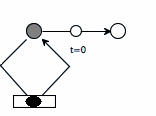
\includegraphics[width=.5\linewidth]{img/bch-timer-mapwitnew}
%   \caption{Mapping of timer event}
%   \label{fig:sub1}
% \end{sub figure}%
% \begin{sub figure}{.5\textwidth}
%   \centering
%   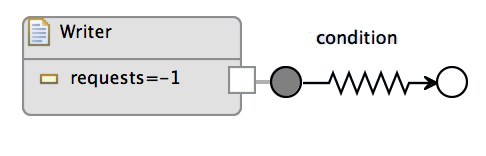
\includegraphics[width=.7\linewidth]{img/bch-img-condition-mapwit}
%   \caption{Mapping of conditional event}
%   \label{fig:sub2}
% \end{sub figure}
% \caption{Translation timer and conditional events}
% \label{fig:timermap}
% \end{figure}
\subsection{Gateway}
The behavior of a {parallel gateway} is determined by the number of its incoming and outgoing sequence flows. If it has only one {incoming sequence flow}, it acts similar to a Reo {replicate} node. If the number of {incoming sequence flows} is more that one, the behavior of the gateway is as of a Reo {join} node as it merges the data items from all the incoming sequence flows and writes the result on the {outgoing sequences flow}s. 

The rule in Listing \ref{lst:gwpar} generates a Reo {node} for the matched {parallel gateway}, wherein the number of incoming {sequence flows} of the gateway determines the type of the generated Reo {node}.

A diverging {inclusive gateway} directs the incoming sequence flow to its outgoing sequences, whose conditions are evaluated to \emph{true}. We can achieve the same behavior using a {replicate} node whose {sink end}s are connected to {filter} channels. Each {filter} channel and its {expression} corresponds to one of the outgoing sequence flows of the gateway. If the condition is met, then the {filter} channel passes the incoming data item through. Otherwise,  the channel loses the data item. Listing \ref{lst:gwinclus} shows the rules that carry out the mapping of the {inclusive gateway} and its outgoing sequence flows.

\begin{lstlisting}[float,frame=single,caption=Mapping inclusive gateway,label=lst:gwinclus]
rule mapInclusiveGateway {
   form
      gwy : BPMN2!InclusiveGateway
   to
      nod : Reo!Node(name <- gwy.name)
}

rule mapSequenceFlowOutOfInclusiveGateway {
   from
     seq : BPMN2!SequenceEdge(seq.sourceRef.oclTypeOf(BPMN2!InclusiveGateway))
   to
     fil : Reo!Filter(sourceEnds <- sce, sinkEnds <- ske, expressions <- seq.sourceRef.condition),
     sce : Reo!SourceEnd(node <- seq.sourceRef),
     ske : Reo!SinkEnd(node <- seq.targetRef)
}
\end{lstlisting}

A diverging {exclusive gateway} creates alternative paths, where only one path can be taken. Similar to an {inclusive gateway}, we map an exclusive gateway using a Reo {router} node and a {filter channel} for each outgoing sequence flow. %However, to ensure that one and only one output path is active we need to check if each condition is met.why not a router We add a {sync drain} to  allow a path to be taken only when the related condition is met. 
 Listing \ref{lst:gw1} presents the rule for mapping an {exclusive gateway} and its outgoing sequence flows.

\begin{lstlisting}[float,frame=single,caption=Mapping exclusive gateway,label=lst:gw1]
rule mapExclusiveGateway {
   form
      gwy : BPMN2!ExclusiveGateway
   to
      nod : Reo!Node(name <- gwy.name, type <- #ROUTE)
}

rule mapSequenceFlowOutOfExclusiveGateway {
   from
     seq : BPMN2!SequenceEdge(seq.sourceRef.oclIsTypeOf(BPMN2!ExclusiveGateway))
   to 
     fil : Reo!Filter(sourceEnds <- src, sinkEnds <- snk, expressions <- seq.sourceRef.condition),
     src : Reo!SourceEnd(node <- seq.sourceRef),
     snk : Reo!SinkEnd(node <- seq.targetRef)
}   
\end{lstlisting}

\subsection{Transaction}
In Listings \ref{lst:nrefine}, \ref{lst:nrefine2}, and \ref{lst:nrefine3}, we have presented an algorithm to refine BPMN 2 transactions, which introduces two kinds of {complex gateway}s.
%with specific conditions allowing flow on its outgoing sequence if either all of its incoming sequence are active or the first two of them. These conditions ensures

\begin{enumerate}
 \item The compensation order complex gateway that ensures that an {activity} is only compensated if a {cancel event} has occurred and the {activity} has been executed, and in case that there is an {activity} that needs to be compensated before this {activity}, it has been compensated.     
 \item The post compensation complex gateway, which prevents that the outgoing sequence flow of the cancel boundary event is taken before all compensation tasks within the given transaction are completed.
\end{enumerate}

 For simplicity, we assume that the transaction refinement step provides a list of the generated complex gateways. Here, we use $orderComplexGateways$ and $postComplexGateway$ to represent these complex gateways. Alternatively, we could detect them programmatically based on their context in terms of their adjacent elements. 
 
 Listing \ref{lst:complexgwtype1} presents the rule for mapping a compensation order {complex gateway}. In this rule and the followings, we capitalize some labels to make it easier to find them later in the figures and to track their usage cross rules. The helper {connectingNode} defined in Listing \ref{lst:fromcomplexgwtype1hlpr} is used in the mapping of incoming sequence flows to compensation order {complex gateway} to connect each incoming sequence to its corresponding node that is generated from the complex gateway. Listing \ref{lst:fromcomplexgwtype1} demonstrates mappings for the sequence flows of the complex gateway.  
 
 To make these rules easier to be understood, Figure \ref{fig:mapcomplexgw1} illustrates the result of applying them to control the flow for compensating the compensatable Task$_i$ with the following compensatable Task$_{i+1}$.

 Listing \ref{lst:complexgw} shows the rule, which maps the post compensation complex gateway to a join node in Reo. The complex gateway incoming sequence from the catching cancel event is presented in Listing \ref{lst:complexgwcancel}. Listings \ref{lst:complexgwtaska} and \ref{lst:complexgwtaskb}, presents rules, which map the gateway incoming sequence flows from the events signalling the task compensation and the task completion, respectively. Due to lengthiness of these rules, in Figure \ref{fig:mapcomplexgw2}, we visualize the result of applying them on a transaction with two compensatable tasks: $Task_i$ and $Task_j$ that are in parallel path without any other compensatable tasks ahead of them in a sequence. 

\begin{lstlisting}[float,frame=single,caption=Mapping the generated compensation order complex gateway,label=lst:complexgwtype1]
rule mapCompensationOrderComplexGateway {
   from
      cxg : BPMN2:ComplexGateway(thisModule.orderComplexGateways->includes(cxg))
   to
      A : Reo!Node(type <- #ROUTE),
      pab : Reo!PrioritySync(sourceEnds <- sca, sinkEnds <- skb),
      sca : Reo!SourceEnd(node <- A),
      skb : Reo!SinkEnd(node <- B),
      B : Reo!Node(type <- #JOIN),
      fbc : Reo!FIFO(sourceEnds <- scb, sinkEnds <- skc),
      scb : Reo!SourceEnd(node <- B),
      skc : Reo!SinkEnd(node <- C),
      C : Reo!Node(type <- #JOIN),
      fcd : Reo!FIFO(sourceEnds <- scc, sinkEnds <- skd),
      scc : Reo!SourceEnd(node <- C),
      skd : Reo!SinkEnd(node <- D),
      D : Reo!Node(type <- #JOIN),
      sae : Reo!SyncDrain(sourceEnds <- Sequence{sra, sre}),
      sra : Reo!SourceEnd(node <- A),
      sre : Reo!SourceEnd(node <- E),
      E : Reo!Node,
      sef : Reo!Sync(sourceEnds <- sce, sinkEnds <- skf),
      sce : Reo!SourceEnd(node <- E),
      skf : Reo!SinkEnd(node <- F),
      F : Reo!SinkEnd(node <- F),
      pdf : Reo!Sync(sourceEnds <- srd, sinkEnds <- snf),
      srd : Reo!SourceEnd(node <- D),
      snf : Reo!SinkEnd(node <- F)
      do {
         for (e in Sequence{pab, fbc, fcd, pdf, sae) {       
            A.connector.primitives.add(e);
         }
      }
}
\end{lstlisting}

\begin{lstlisting}[float,frame=single,caption=Finding the connecting node to a complex gateway,label=lst:fromcomplexgwtype1hlpr]
helper context BPMN2!FlowNode def : connectingNode(gw : ComplexGateway) : String =
   if self.oclTypeOf(BPMN2!CatchingCancelEvent)
   then 'A'
   else if self.oclTypeOf(BPMN2!CatchingSignalEvent)
         then if thisModule.compensatables.get(gw)->includes(self)  
              then 'B'
              else if thisModule.nextCompensatables.get(gw)->includes(self)
                    then 'C'
                    else if thisModule.nextCompensations.get(gw)->includes(self)
                           then 'D'
                         endif  
                    endif
              endif
         else 'UNKNOWN'
   endif;
\end{lstlisting}
 

\begin{lstlisting}[float,frame=single,caption=Mapping incoming flows of the compensation order gateway,label=lst:fromcomplexgwtype1]
rule mapSequenceFlowFromCompensatableToOrderComplexGateway {
   from
      seq : BPMN2!SequenceFlow(thisModule.orderComplexGateways->includes(seq.targetRef) and thisModule.nextCompensations.get(gw)->includes(seq.sourceRef))
   to 
      fia : Reo!FIFO(sourceEnds <- sca, sinkEnds <- ska),
      sca : Reo!SourceEnd(node <- seq.sourceRef),
      ska : Reo!SinkEnd(node <- thisModule.resolveTemp(seq.targetRef, seq.sourceRef.connectingNode(seq.targetRef))),
      blk : Reo!BlockSync(sourceEnds <- scb, sinkEnds <- skb),
      scb : Reo!SourceEnd(node <- seq.sourceRef),
      skb : Reo!SinkEnd(node <- thisModule.resolveTemp(seq.targetRef, 'E'))
}

rule mapSequenceFlowToOrderComplexGateway {
   from
      seq : BPMN2!SequenceFlow(thisModule.orderComplexGateways->includes(seq.targetRef) and not thisModule.nextCompensations.get(gw)->includes(seq.sourceRef))
   to 
      fia : Reo!FIFO(sourceEnds <- sca, sinkEnds <- ska),
      sca : Reo!SourceEnd(node <- seq.sourceRef),
      ska : Reo!SinkEnd(node <- thisModule.resolveTemp(seq.targetRef, seq.sourceRef.connectingNode(seq.targetRef)))
}

rule mapSequenceFlowFromOrderComplexGateway {
   from
      seq : BPMN2!SequenceFlow(thisModule.orderComplexGateways->includes(seq.sourceRef))
   to refined 
      syn : Reo!Sync(sourceEnds <- src, sinkEnds <- snk),
      src : Reo!SourceEnd(node <- thisModule.resolveTemp(seq.sourceRef, 'F')),
      snk : Reo!SinkEnd(node <- seq.targetRef)
}
\end{lstlisting}

\begin{figure}[t!]
  \centering
  \scalebox{.85}{
\begin{tikzpicture}[line cap=round,line join=round,>=triangle 45,x=1cm,y=1cm]
%labels
    \node[rotate=-90,label={[shift={(-.5,1.1)}]A}] at (1, -.6)   (b) {!};
    \node[rotate=-90,label={[shift={(.2,-.9)}]B}] at (1, -.6)   (b) {};
    \node[rotate=-90,label={[shift={(.2,-2.4)}]C}] at (1, -.6)   (b) {};
    \node[label={[shift={(-1.2,-1.1)}]D}] at (2.25, -4.5)   (b) {)(};
  %  \node[] at (2.5, -5.6)   (b) {)(};
    \node[] at (-2.35, .5)   (b) {Cancel};
    \node[] at (-2, -1)   (b) {Task$_{i+1}$ done};
    \node[] at (-1.8, -2.55)   (b) {Task$_{i+1}$ compensated};
    \node[] at (-2, -4)   (b) {Task$_{i}$ done};
    \node[] at (3.5, .5)   (b) {E};
    \node[] at (4, -4.5)   (b) {F};
    \node[] at (4, -5)   (b) {Task$_i$ to be compensated};
%%%%%%%%
\draw [line width=1.2pt] (-1.25*2,0) circle (0.2cm);%xel
\draw [line width=1.2pt] (-.25*2,0) circle (0.2cm);%xel
\draw [line width=1.2pt] (.5*2,0) circle (0.2cm);%X
\draw [line width=1.2pt] (-1.25*2,-1.5) circle (0.2cm);%done
\draw [line width=1.2pt] (-.25*2,-1.5) circle (0.2cm);%done
\draw [line width=1.2pt] (-1.25*2,-3) circle (0.2cm);%predone
\draw [line width=1.2pt] (-.25*2,-3) circle (0.2cm);%predone
\draw [line width=1.2pt] (-1.25*2,-4.5) circle (0.2cm);%preundone
\draw [line width=1.2pt] (-.25*2,-4.5) circle (0.2cm);%preundone
\draw [line width=1.2pt] (1.75*2,0) circle (0.2cm);%no compensation needed
%%%%col2
%\draw [line width=1.2pt] (6,0) circle (0.2cm);%last
%done
\draw [line width=1.2pt] (2.5-.75*2,-3) circle (0.2cm);%predone
\draw [line width=1.2pt] (2.5-.75*2,-4.5) circle (0.2cm);%preundone
\draw [line width=1.2pt] (2.5-.75*2,-1.5) circle (0.2cm);%xel
%%%+ 3
\draw [line width=1.8pt] (.99, -3.2) -- (.99,-2.8);
\draw [line width=1.5pt] (.82, -3) -- (1.2,-3);
%%%+ 2
\draw [line width=1.8pt] (.99, -4.7) -- (.99,-4.3);
\draw [line width=1.5pt] (.82, -4.5) -- (1.2,-4.5);
%%%+ 1
\draw [line width=1.8pt] (.99, -1.7) -- (.99,-1.3);
\draw [line width=1.5pt] (.82, -1.5) -- (1.2,-1.5);
%%col3
\draw [line width=1.2pt] (5-.75*2,-4.5) circle (0.2cm);%+el 3
%%%X
\draw [line width=1.5pt] (.9, -.1) -- (1.1,.1);
\draw [line width=1.5pt] (.9, .1) -- (1.1,-.1);
%%%lines1
\draw [->, thick] (-2.3,0) -- (-.7,0);%1 cancel to X
\draw [->, thick] (-.3,0) -- (.8,0);%1 cancel to X
\draw [->, thick] (-2.3,-1.5) -- (-.7,-1.5);%2
\draw [->, thick] (-.3,-1.5) -- (.8,-1.5);%2
\draw [->, thick] (-2.3,-3) -- (-.7,-3);%3
\draw [->, thick] (-.3,-3) -- (.87,-3);%3
\draw [->, thick] (-2.3,-4.5) -- (-.7,-4.5);%4
\draw [->, thick] (-.3,-4.5) -- (.87,-4.5);%4
\draw [->, thick] (1.2,0) -- (2.25,0);%syncdrain
\draw [->, thick] (3.3,0) -- (2.25,0);%syncdrain
\draw [->, thick] (5.8,0) -- (3.7,0);%faghat do ta
\draw [->, thick] (3.5,-.2) -- (3.5,-4.3);%faghat do ta amudi
%% X to + amoodi.
\draw [-, thick] (-.5,-4.7) -- (-.5,-5.6) -- (6, -5.6) -- (6,-5.6) -- (6,0) -- (5.7,0);%khaat
\draw [->, thick] (1,-.2) -- (1,-1.3);%2
%% khali to + 
\draw [->, thick] (1.2,-4.5) -- (3.3,-4.5);%3ifo
%fifo
\fill[white, draw=black, very thick] (-1.75,.1) rectangle (-1.25,-.1);%fifo balatarintar
%\fill[white, draw=black, very thick] (5-.55,.1) rectangle (5-.05,-.1);%fifo balatarintar
\fill[white, draw=black, very thick] (-1.75,-1.4) rectangle (-1.25,-1.6);%fifo balatarin
\fill[white, draw=black, very thick] (-1.75,-2.9) rectangle (-1.25,-3.1);%fifo bala
\fill[white, draw=black, very thick] (-1.75,-4.4) rectangle (-1.25,-4.6);%fifo paiin
\draw [->, thick] (1,-1.7) -- (1,-2.8);
%%line 3 to four
\draw [->, thick] (1,-3.2) -- (1,-4.3);
\fill[white, draw=black, very thick] (.9,-1.9) rectangle (1.1,-2.4);%fifo amudi
%%line 2 to three
\fill[white, draw=black, very thick] (.9,-3.4) rectangle (1.1,-3.9);%fifo amudi
%%line 2 to three
        \node[] at (.1, -4.5)   (b) {$!$};
        %%%X
\draw [line width=1.5pt] (.9-1.5, -4.5-.1) -- (1.1-1.5,-4.5+.1);
\draw [line width=1.5pt] (.9-1.5, -4.5+.1) -- (1.1-1.5,-4.5-.1);
%%%+ 
\draw [line width=1.8pt] (.99, -4.7) -- (.99,-4.3);
\draw [line width=1.5pt] (.82, -4.5) -- (1.2,-4.5);
\end{tikzpicture}
}
\caption{Mapping of the compensation order complex gateway}
\label{fig:mapcomplexgw1}
\end{figure}

\begin{lstlisting}[float,frame=single,caption=Mapping the post compensation complex gateway,label=lst:complexgw]
rule mapPostCompensationComplexGateway {
   from
      cxg : BPMN2:ComplexGateway(cxg = thisModule.postComplexGateway)
   to
      G : Reo!Node(type <- #JOIN)
}
\end{lstlisting}

\begin{lstlisting}[float,frame=single,caption=Mapping the cancel flow to the post compensation gateway,label=lst:complexgwcancel]  
rule mapCancelToPostCompensationComplexGatewaySequenceFlow {
   from
      seq : BPMN2!SequenceFlow(seq.sourceRef.oclTypeOf(BPMN2!CatchingCancelEvent)  and seq.targetRef = thisModule.postComplexGateway)
   to 
      fia : Reo!FIFO(sourceEnds <- sca, sinkEnds <- ska),
      sca : Reo!SourceEnd(node <- seq.sourceRef),
      ska : Reo!SinkEnd(node <- F),
      F : Reo!Node
}
\end{lstlisting}


\begin{lstlisting}[float,frame=single,caption=Mapping the compensation completion,label=lst:complexgwtaska]  
rule mapCompensationToPostCompensationGatewaySequenceFlow {
   from
      seq : BPMN2!SequenceFlow(seq.targetRef = thisModule.postComplexGateway and seq.sourceRef.oclIsKindOf(BPMN!CatchingSignalEvent) and thisModule.nextCompensations.get(seq.targetRef)->includes(seq.sourceRef))
   to
      fi1 : Reo!FIFO(sourceEnds <- sc1, sinkEnds <- sk1),
      sc1 : Reo!SourceEnd(node <- seq.sourceRef),
      sk1 : Reo!SinkEnd(node <- A),
      A   : Reo!Node(type <- #JOIN),
      fi2 : Reo!FIFO(sourceEnds <- sc2, sinkEnds <- sk2),
      sc2 : Reo!SourceEnd(node <- thisModule.resolveTemp(seq.sourceRef, 'C')),
      sk2 : Reo!SinkEnd(node <- A),      
      sab : Reo!Sync(sourceEnds <- sca, sinkEnds <- skb),
      sca : Reo!SourceEnd(node <- A),
      skb : Reo!SinkEnd(node <- B),      
      B   : Reo!Node,
      fi3 : Reo!FIFO(sourceEnds <- sce, sinkEnds <- snb),
      sce : Reo!SourceEnd(node <- thisModule.resolveTemp(seq.sourceRef, 'E')),
      snb : Reo!SinkEnd(node <- B),
      bbg : Reo!BlockSync(sourceEnds <- scb, sinkEnds <- skg),
      scb : Reo!SourceEnd(node <- B),
      skg : Reo!SinkEnd(node <- thisModule.resolveTemp(seq.sourceRef, 'G'))
      do {
            fil.connector.nodes.add(A);
            fil.connector.nodes.add(B);
      }
}
\end{lstlisting}


\begin{lstlisting}[float,frame=single,caption=Mapping the task completion,label=lst:complexgwtaskb]  
rule mapCompensatableToPostCompensationGatewaySequenceFlow {
   from
      seq : BPMN2!SequenceFlow(seq.targetRef = thisModule.postComplexGateway and
      seq.sourceRef.oclIsKindOf(BPMN!CatchingSignalEvent) and
             thisModule.nextCompensatables.get(seq.targetRef)->includes(seq.sourceRef))
   to
      fic : Reo!FIFO(sourceEnds <- scf, sinkEnds <- skc),
      scf : Reo!SourceEnd(node <- seq.sourceRef),
      skc : Reo!SinkEnd(node <- C),
      C   : Reo!Node,
      pri : Reo!PrioritySync(sourceEnds <- scc, sinkEnds <- skd),
      scc : Reo!SourceEnd(node <- ndc),
      skd : Reo!SinkEnd(node <- D),
      D   : Reo!Node,
      sdr : Reo!SyncDrain(sourceEnds <- Sequence{scf, scd}),
      scf : Reo!SourceEnd(node <- thisModule.resolveTemp(seq.targetRef, 'F')),
      scd : Reo!SourceEnd(node <- D),
      syn : Reo!Sync(sourceEnds <- sec, sinkEnds <- snd),
      snd : Reo!SinkEnd(node <- D),
      sec : Reo!SourceEnd(node <- E),
      E : Reo!Node,
      ffe : Reo!FIFO(sourceEnds <- sen, sinkEnds <- ske, full <- true),
      sen : Reo!SourceEnd(node <- ndt),
      ske : Reo!SinkEnd(node <- D),
      ndt : Reo!Node
      do {
         for (e in Sequence{C, D, E, ndt}) {       
            fic.connector.nodes.add(e);
         }
      }
}
\end{lstlisting}

\begin{figure}[!th]
  \centering
  \scalebox{.85}{
\begin{tikzpicture}[line cap=round,line join=round,>=triangle 45,x=1cm,y=1cm]
    \begin{scope}[shift={(5,0)}]
%labels
    \node[rotate=-30] at (6.4, -1.45) (lp) {)(};
    \node[rotate=30] at (6.6, -4.45) (lp) {)(};
    \node[] at (2.2, -4.5)   (lbp) {$!$};
    \node[] at (2.2, -1.5)   (lbp2) {$!$};
		\node [label={[shift={(-2,-0.4)}]Task$_i$ compensated}] (0) at (0, -0) {};
		\node [label={A$_i$}] (1) at (1.5*1, -0) {};
		\node [label={B$_i$}] (2) at (1.5*3, -0) {};
		\node [label={[shift={(.5,-.25)}]G}] (3) at (1.5*5.5, 1.5*-2) {};
		\node [label={[shift={(-1.5,-.4)}]Task$_i$ done}] (4) at (0, 1.5*-1) {};
		\node [label={[shift={(0,-.8)}]C$_i$}] (5) at (1.5*1, 1.5*-1) {};
		\node [label={D$_i$}] (6) at (1.5*2, 1.5*-1) {};
		\node [label={[shift={(.5,-.3)}]E$_i$}] (7) at (1.5*3, 1.5*-1) {};
		\node [label={[shift={(-1.2,-.4)}]Cancel}] (8) at (0, 1.5*-2) {};
		\node [label={[shift={(.4,-.3)}]F}] (9) at (1.5*2, 1.5*-2) {};
		\node [label={[shift={(1.5,-.4)}]Task$_i$ not done}] (10) at (1.5*3, 1.5*-1.85) {};
		\node [label={[shift={(1.5,-.5)}]Task$_j$ not done}] (11) at (1.5*3, 1.5*-2.15) {};
		\node [label={[shift={(-1.5,-0.4)}]Task$_j$ done}] (12) at (0, 1.5*-3) {};
		\node [label={[shift={(-2,-0.45)}]Task$_j$ compensated}] (13) at (0, 1.5*-4) {};
		\node [label={C$_j$}] (14) at (1.5*1, 1.5*-3) {};
		\node [label={[shift={(0,-.8)}]A$_j$}] (15) at (1.5*1, 1.5*-4) {};
		\node [label={[shift={(0,-.85)}]D$_j$}] (16) at (1.5*2, 1.5*-3) {};
		\node [label={[shift={(0,-.85)}]B$_j$}] (17) at (1.5*3, 1.5*-4) {};
		\node [label={[shift={(.5,-.35)}]E$_j$}] (18) at (1.5*3, 1.5*-3) {};
		
		\draw [->, thick] (0.west) to (1.west);
		\draw [->, thick] (1.center) to (2.west);
		\draw [->, thick] (2.center) to (3.north);%orib
		\draw [->, thick] (17.center) to (3.south);
		\draw [->, thick] (15.center) to (17.west);
		\draw [->, thick] (13.center) to (15.west);
		\draw [->, thick] (12.center) to (14.west);
		\draw [->, thick] (14.center) to (16.west);
		\draw [->, thick] (14.center) to (15.north);%%vertical fifo
		\draw [->, thick] (18.center) to (17.north);%%%%vertical
		\draw [->, thick] (11.center) to (18.north);%%%orib fullfifo
		\draw [->, thick] (10.center) to (7.south);%%%orib barax fullfifo upwards
		\draw [->, thick] (18.center) to (16.east);
		\draw [->, thick] (8.center) to (9.west);
        \draw [->, thick] (3,-3) to (3,-3.82);%%%vertical syncdrain
        \draw [->, thick] (3,-4.5) to (3,-3.7);%%%vertical syncdrain
		\draw [->, thick] (3,-1.5) to (3,-2.3);%%%vertical syncdrain
        \draw [->, thick] (3,-3) to (3,-2.18);%%%vertical syncdrain
        \draw [->, thick] (7.center) to (6.east);
		\draw [->, thick] (5.center) to (6.west);
		\draw [->, thick] (4.center) to (5.west);
		\draw [->, thick] (5.center) to (1.south);%%vertical upward
		\draw [->, thick] (7.center) to (2.south);%%vertical upward
		
       \foreach \i in {0,...,18} 
       {
        \fill[white, draw=black, very thick] (\i) circle (0.15cm);
       } 
       %%%+ node 1
\draw [line width=1.5pt] (1.35, 0) -- (1.65,0);
\draw [line width=1.5pt] (1.5, -.15) -- (1.5,.15);
%%+
\draw [line width=1.5pt] (1.35, -6) -- (1.65,-6);
\draw [line width=1.5pt] (1.5, -6.15) -- (1.5,-5.75);
%%+
\draw [line width=1.2pt] (1.5*5.5-.15, -3) -- (1.5*5.5+.15,-3);
\draw [line width=1.2pt] (1.5*5.5, -3-.15) -- (1.5*5.5,-3+.15);
%fifos
\fill[white, draw=black, very thick] (.85,-.1) rectangle (.45,.1);%row1
\fill[white, draw=black, very thick] (.85,-1.5-.1) rectangle (.45,-1.5+.1);%row2
\fill[white, draw=black, very thick] (1.7,-3-.11) rectangle (1.2,-3+.11 );%row3
\fill[white, draw=black, very thick] (.85,-4.5-.1) rectangle (.45,-4.5+.1);%row4
\fill[white, draw=black, very thick] (.85,-6-.1) rectangle (.45,-6+.1);%row5
%%%vertical fifos
\fill[white, draw=black, very thick] (1.4,-.6) rectangle (1.6,-1);%row1
\fill[white, draw=black, very thick] (4.4,-.6) rectangle (4.6,-1);%row1
\fill[white, draw=black, very thick] (1.4,-4.9) rectangle (1.6,-5.3);%row4
\fill[white, draw=black, very thick] (4.4,-4.9) rectangle (4.6,-5.3);%row4
%%fullfifos
\fill[white, draw=black, very thick] (4.4,-2.45) rectangle (4.6,-2.1);
\fill[black, draw=black, very thick] (4.5, -2.25) circle (0.05cm);
\fill[white, draw=black, very thick] (4.4,-3.9) rectangle (4.6,-3.6);
\fill[black, draw=black, very thick] (4.5, -3.75) circle (0.05cm);
\end{scope}
\end{tikzpicture}
}
\caption{Mapping of the post compensation complex gateway}
\label{fig:mapcomplexgw2}
\end{figure}

\subsection{Other elements}
In general, we map sequence flows to {sync} channels that coordinate the mapped elements. We map the rest of BPMN 2 flow nodes that are not mapped by the aforementioned rules to Reo nodes.

Since ATL does not provide a mechanism to provide priority over the rules, the rule for mapping the non-specific elements need to have a condition to assure that they do not match any of the existing rules. This is simply achieved by negating the disjunction of the related rules. %We use  helpers to find the source and sink of the generated sync channel to be passed to the $resolveTemp$ operator. The \emph{resolveTemp} operator enables referencing a target element that is created during mapping. 
%
%The rule in Listing \ref{lst:proc2conn} assigns the result of mapping a {flowNode} to the node sets of a Reo connector. Note that the \emph{sourceRef} and \emph{targetRef} attributes of a sequence flow refer to its source and target flow node (defined in rule \ref{}). 
%
%\begin{lstlisting}[float,frame=single, caption=Mapping the incoming sequence flow to a task and a collapsed subprocess,label=lst:]
%rule mapTaskAndCollapsedSubprocessIncomingSequence {
 %   from 
  %    seq : BPMN2!SequenceFlow(seq.targetRef.oclIsKindOf(BPMN2!Task) or (seq.targetRef.oclIsKindOf(BPMN2!SubProcess) and not seq.targetRef.expandedSubProcess()))
   % to
    %  sy1 : Reo!Sync(src, snk),
     % src : Reo!SourceEnd(node <- seq.sourceRef),
      %snk : Reo!SinkEnd(node <- thisModule.resolveTemp(seq.targetRef, 'ndc')))
% }
%\end{lstlisting}
%
%
%\begin{lstlisting}[float,frame=single, caption=Mapping a sequence flow,label=lst:subprocseq]
%helper cotext BPMN2!SequenceFlow sourceOrigin 
 % if (self.sourceRef.oclIsKindOf(BPMN2!Task)) or BPMN2!SequenceFlow(self.sourceRef.oclIsKindOf(BPMN2!SubProcess));
%helper cotext BPMN2!SequenceFlow sinkOrigin;
%helper cotext BPMN2!SequenceFlow reoNodeType;
%
%rule mapSequenceFlow {
 %   from
  %    seq : BPMN2!SequenceFlow
   % to
    %   syn : Reo!Sync(sourceEnds <- src, sinkEnds <- snk),
     %  src : Reo!SourceEnd(node <- rtr),
      % snk : Reo!SinkEnd(node <- seq.targetRef),
       %rtr : Reo!Node(type <- #ROUTE),
       %
%    do {
 %       syn.connector.nodes.add(rtr);
  %  }
 %}
%\end{lstlisting}

\begin{figure}[!th]
\centering 
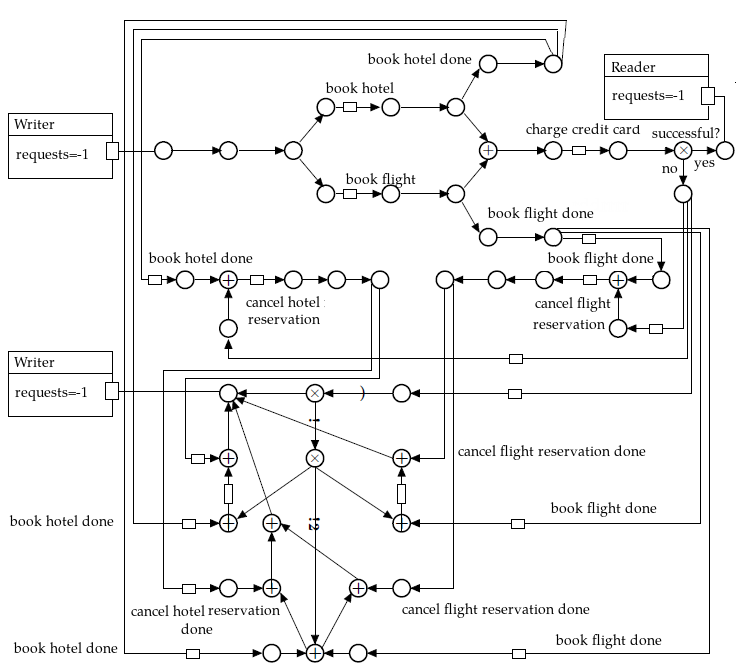
\includegraphics[width=1\textwidth]{img/exampleb2r.png} 
\caption{Mapping the refined BPMN 2 example of Figure \ref{fig:baxtionref} to Reo} 
\label{fig:finalreoex} 
\end{figure}

\section{Example}
\label{exmap}
Figure \ref{fig:finalreoex} shows the result of applying the presented BPMN 2 to Reo transformation rules on the refined  BPMN 2 model of Figure \ref{fig:baxtionref}.

%\afterpage{\clearpage}
%\newpage
\vspace*{.2cm}
\section{Related Work}
\label{chapterconv:relwrk}
Several works on the topic of formal semantics of business processes propose a mapping from BPMN to Petri nets \cite{journalsjcscAalst98} e.g. \cite{Tantitharanukul2010DetectingDA}, \cite{whyformalbpmn}, \cite{Decker11}, and \cite{doi:10.1177/1687814018808170}.
 Petri nets constitute a graph-based modeling language for describing distributed systems. Similar to BPMN, Petri nets have a graphical syntax and its execution
semantics have exact mathematical definitions. 

The obtained Petri nets model can be analyzed using Petri nets analyzing tools such as ProM \cite{10.10071149474425}, Yasper
\cite{yasperrr}, Woflan \cite{DBLP:journals/itm/VerbeekAK04}, Snoopy\cite{10.1007/978-3-642-31131-422}, and CPN Tools \cite{DBLP:journals/sttt/JensenKW07}. Each of these tools performs
particular types of analyses. Some tools can only analyze a subset of Petri nets.

Groote et al. in  \cite{mcrl2} propose converting the obtained Petri nets models to
the process specification language mCRL2 to open up the possibility of
automatic verification by the mCRL2 tool-set.

Alternatively, BPMN has been mapped to other formalisms. Wong et al.
\cite{Wong2008APS} propose a mapping from BPMN to Communicating Sequential Processes
(CSP) \cite{Hoare:1985:CSP:3921}, a type of process algebra.  

Christiansen et al. \cite{101007978364219589110} use a token-based semantics to define formal semantics for BPMN processes. Authors of
\cite{20142630768} propose a formal semantics for BPMN processes in Maude \cite{DBLPjournalstcsClavelM02}, a logical
declarative language based on rewriting logic.  Prandi et al. \cite{PrandiQZ08} suggest a
translation of BPMN into the process algebra COWS \cite{cows}. 

Braghetto et al. in
\cite{braghetto:hal-00788815} propose a mapping of BPMN processes into Stochastic Automata Network
(SAN) \cite{DBLP:journals/tse/PlateauA91} - a compositionally built stochastic model. Authors of \cite{Mateescu14bpmn} present
a formal model for BPMN processes in terms of Labelled Transition Systems,
which are obtained from process algebra encoding. Poizat et al. in \cite{Poizatrealize} propose
a model transformation into the LOTOS NT process algebra \cite{Garavel2017}.

A drawback of using aforementioned formalisms compared to Petri nets is
that they do not preserve the structure of the original BPMN model, as they
are lower level languages and at finer granularity compared to BPMN.
Reo has graphical syntax and exact mathematical definitions of its execution
semantics. It defines a form of coordination in terms of synchronizing, buffering, retaining data, etc., along with constraining its input and output data
items. Reo allows hierarchical modeling where arbitrarily complex models can
be formed out of simpler ones. 

The semantics of Reo is compositional. This
means that complex networks can be built by connecting simpler networks.
 Once a business model is transformed to a Reo network, its behavior can
be formally studied using various programs within the Extensible Coordination
Tools (ECT) \cite{ect}, a set of Eclipse plug-ins that constitute an integrated development environment for the Reo coordination language. 

ECT contains tools for the design \cite{ect}, animation \cite{Krause11a}, simulation \cite{oscarmaster}, testing \cite{aichernig2009fault}, stochastic analysis \cite{ArbabCMM07}, verification \cite{Kppelholz2009688, KKdV10areo,Mousavi04-ReoTechRep}, execution \cite{JoseThesis,SFM-2015-ArbabJ,ect,Jongmans2012}, and model transformation \cite{behnaz,TVM+08,Krause201123} for Reo networks. 
